\documentclass{beamer}

\usetheme{Warsaw}
\usecolortheme{orchid}

\usepackage{algorithm,algorithmic}
\usepackage{amssymb}
\usepackage{amsthm}
\usepackage{pgfplots} 
\usepackage{graphicx}
\usepackage[utf8x]{inputenc}
\usepackage{tikz}
\usepackage{bbm}
\usepackage{subcaption}
\usepackage{mathtools}
\usepackage{lipsum}
\usepackage{color}
\usepackage{}
\DeclarePairedDelimiter{\ceil}{\lceil}{\rceil}
\newcommand{\eqtext}[1]{\ensuremath{\stackrel{#1}{=}}}
\newcommand{\leqtext}[1]{\ensuremath{\stackrel{#1}{\leq}}}
\newcommand{\N}{\mathbb{N}}
\newcommand{\R}{\mathbb{R}}
\newcommand{\E}{\mathbb{E}}
\newcommand{\epl}{\varepsilon}
\newcommand{\defeq}{\coloneqq}
\newcommand{\uDarcy}{\color{red}{u}}
\newtheorem{proposition}[theorem]{Proposition}
\renewcommand{\phi}{\varphi}
\definecolor{mygray}{gray}{0.8}

% Add numbers and take out navigation symbols
\setbeamertemplate{footline}[frame number]
\beamertemplatenavigationsymbolsempty

\title{Uncertain Darcy's problem \\ and the stochastic particle transport}
\subtitle{Semester Project - Master in CSE}
\author{Giacomo Garegnani \\ {Supervisors: Dr. Sebastian Krumscheid and Prof. Fabio Nobile}}
\institute{EPFL}
\date{16/06/2016}

\begin{document}

\frame{\titlepage}

\begin{frame}
\frametitle{Problem statement}
Underground flow $\rightarrow$ Uncertain Darcy's problem
\begin{equation*}
	\left \{
  	\begin{aligned}
		\uDarcy &= -A \nabla p, && \text{in } D, \\
		\nabla\cdot \uDarcy &= f, && \text{in } D, \\
		p &= p_0, && \text{on } \Gamma_{in},\\
		p &= 0, && \text{on } \Gamma_{out}, \\
		\nabla p \cdot n &= 0, && \text{on } \Gamma_N.
	\end{aligned} \right.
\end{equation*}
Stochastic particle transport $\rightarrow$ SDE
\begin{equation*}
	\left \{
	\begin{aligned}
		dX(t) &= \uDarcy (X(t)) \color{black} dt + \sigma dW(t), && 0 \leq t \leq T, \\
		X(0) &= X_0 \in D, \\
	\end{aligned} \right.
\end{equation*}
\end{frame}

\begin{frame}
\frametitle{Outline of the presentation}
\begin{itemize}
	\item Expected exit time from a domain
	\begin{itemize}
		\item[--] Setting
		\item[--] Numerical methods
		\item[--] Numerical experiments
	\end{itemize}
	\item Theoretical investigation: perturbed SDE's 
	\item The uncertain Darcy's problem 
\end{itemize}
\end{frame}

\begin{frame}
\frametitle{Mean exit time. Setting}
Given a domain $D \subset \R^d$, $f\colon D \to \R^d, g\colon D \to \R^{d \times m}$ and an $m$-dimensional standard Wiener process $W(t)$, consider
\begin{equation*}
\left \{
\begin{aligned}
	dX(t) &= f(X(t)) dt + g(X(t))dW(t), && 0 < t \leq T, \\
	X(0)  &= X_0, && X_0 \in D.
\end{aligned} \right .
\end{equation*}
The equation is defined in a domain $D$ $\rightarrow$ boundary conditions
\begin{itemize}
	\item \textit{killing boundaries}: $X(t)$ is stopped,
	\item \textit{reflecting boundaries}: $X(t)$ is reflected normally inside $D$.
\end{itemize}
\end{frame}

\begin{frame}
\frametitle{Mean exit time. Problem statement}
\underline{Problem}. Estimate the exit time of the trajectories
\begin{equation*}
	\tau = \min\{\tau_e,T\}, \text{ where } \tau_e = \min\{t\colon X(t)\notin D\}.
\end{equation*}
Another quantity of interest, given $F\colon D \to \R$
\begin{equation*}
	\phi = \phi(T,X_0,F) = \mathbbm{1}_{\{T < \tau_e\}}F(X(T)).
\end{equation*}
If $F \equiv 1$, exit probability 
\begin{equation*}
	\Phi(T,X_0) \defeq \Pr(\tau < T | X(0) = X_0) = 1 - \mathbb{E}(\phi(T,X_0,1)). 
\end{equation*}
\underline{Goal}. Estimate numerically $\tau$ and $\phi$.
\end{frame}

\begin{frame}[plain]
\frametitle{Discrete Euler-Maruyama}
Method:
\begin{equation*}
	\left \{
	\begin{aligned}
		X_h^d(t_{i+1}) &= f(X(t_i))h + g(X(t_i))(W(t_{i+1}) - W(t_{i})),  \\
		X_h^d(0) &= X_0.
	\end{aligned} \right .
\end{equation*}
Parameters of interest computed naively
\begin{equation*}
\begin{aligned}
	\tau_h^d &= \min\{\tau_{h,e}^d,T\}, \text{ where } \tau_{h,e}^d = \min \{t_i \colon X_h^d(t_i) \notin D\}, \\
	\phi_h^d &= \mathbbm{1}_{\{T < \tau_{h,e}^d\}}F(X_h^d(T)).
\end{aligned}
\end{equation*}
Missed exits $\Rightarrow$ 1/2 loss in weak order:
\begin{align*}
	|\mathbb{E}(\tau_h^d) - \mathbb{E}(\tau)| &= O(\sqrt{h}), \\
	|\mathbb{E}(\phi_h^d) - \mathbb{E}(\phi)| &= O(\sqrt{h}).
\end{align*}	
\end{frame}

\begin{frame}[plain]
\frametitle{Continuous Euler-Maruyama}
\underline{Goal}. Restore the order of convergence 1 of Euler-Maruyama in $\R^d$ $\Rightarrow$ Brownian bridge approach.

Method:
\begin{equation*}
	\left \{
	\begin{aligned}
		X_h^c(t) &= f(X(t_i))(t-t_i) + g(X(t_i))(W(t) - W(t_{i})),  && t_i < t \leq t_{i+1},\\
		X_h^c(0) &= X_0.
	\end{aligned} \right .
\end{equation*} 
Estimate at each time step the probability of exit. If $D$ is an half-space
\begin{equation*}
\begin{aligned}
	&\Pr (\exists t \in [ t_i,t_{i+1} ] \quad X_h^d(t) \notin D | X_h^d(t_i) = x_i, X_h^d(t_{i+1}) = x_{i+1}) \\
	&\quad = p(x_i,x_{i+1},h) \\
	&\quad = \exp\Big(-2\frac{[n\cdot(x_i - z_i)][n\cdot(x_{i+1} - z_i)]}{hn\cdot (gg^T(x_i)n)}\Big),
\end{aligned}
\end{equation*}
\end{frame}

\begin{frame}
\frametitle{Continuous Euler-Maruyama}
Parameters of interest. Given $u$ a realization of $U$ uniform r.v. in $(0,1)$
\begin{equation*}
\begin{aligned}
	\tau_h^c &= \min \{T,\tau_{h,e}^c\}, \\
	\text{ where } \tau_{h,e}^c &= \min\{\tau_{h,e1}^c, \tau_{h,e2}^c\}, \\
	\tau_{h,e1}^c &= \min\{t_i = hi \colon X_h(t_i) \notin D\}, \\
	\tau_{h,e2}^c &= \min\{t_i = hi \colon u < p(x_{i-1},x_i,h) \}, \\
	\phi_h^c &= \mathbbm{1}_{\{T < \tau_{h,e}^c\}}F(X_h^c(T)).
\end{aligned}
\end{equation*}
Weak order 1 is restored:
\begin{align*}
	|\mathbb{E}(\tau_h^c) - \mathbb{E}(\tau)| &= O(h), \\
	|\mathbb{E}(\phi_h^c) - \mathbb{E}(\phi)| &= O(h).
\end{align*}
\end{frame}


\begin{frame}
\frametitle{Outline of the presentation}
\begin{itemize}
	\item \color{mygray} Expected exit time from a domain
	\begin{itemize} \color{mygray}
		\item[--] Setting
		\item[--] Numerical methods
		\item[--] Numerical experiments
	\end{itemize} \color{black}
	\item Theoretical investigation: perturbed SDE's 
	\item The uncertain Darcy's problem 
\end{itemize}
\end{frame}

\begin{frame}
\frametitle{Theoretical investigation - Motivation}
Consider the velocity field $\uDarcy$ solution of the Darcy's problem and an approximation $\color{blue} \tilde u$ of $\uDarcy$. Consider then the SDE
\begin{equation*}
	\left \{
	\begin{aligned}
		dX(t) &= \uDarcy (X(t)) \color{black} dt + \sigma dW(t), && 0 \leq t \leq T, \\
		X(0) &= X_0 \in D, \\
	\end{aligned} \right.
\end{equation*}
and the SDE
\begin{equation*}
	\left \{
	\begin{aligned}
		d\tilde X(t) &= \color{blue} \tilde u(\tilde X(t)) \color{black} dt + \sigma dW(t), && 0 \leq t \leq T, \\
		\tilde X(0) &= X_0 \in D, \\
	\end{aligned} \right.
\end{equation*}
\underline{Problem}. If $\color{blue} \tilde u$ converges to $\uDarcy$, does $\tilde X(t)$ converge to $X(t)$? What is the effect on the order of convergence of numerical methods?
\end{frame}

\begin{frame}
\frametitle{Theoretical investigation - Convergence of the solution}
In an abstract form, consider $f\colon \R \to \R$ and the SDE
\begin{equation*}
\left \{
\begin{aligned}
	dX(t) &= f(X(t))dt + \sigma dW(t), && 0 < t \leq T, \\
	X(0) &= X_0,
\end{aligned} \right .
\end{equation*}
Consider a perturbation of the transport field $f^\epl\colon \R \rightarrow \R$ and
\begin{equation*}
\left \{
\begin{aligned}
	dX^\epl(t) &= f^\epl(X^\epl(t))dt + \sigma dW(t), && 0 < t \leq T, \\
	X^\epl(0) &= X_0.
\end{aligned} \right .
\end{equation*}

\end{frame}

\begin{frame}
\frametitle{Theoretical investigation - Convergence of the solution}
\begin{proposition} If the following assumptions are verified for a constant $K > 0$
\begin{enumerate}
	\item $|f(x) - f(y)| \leq K|x - y|, \: \forall x,y \in \R$,
	\item $|f(x)| \leq K(1 + |x|), \: \forall x \in \R$,
\end{enumerate}
and if the solution $X^\epl(t)$ of the perturbed SDE exists, then
\begin{equation*}
	\E \sup_{0 \leq t \leq T} |X^\epl(t) - X(t)|^2 \leq  2T^2 \|f - f^\epl\|_{\infty}^2 e^{2K^2T^2}.
\end{equation*}
\end{proposition}
\underline{Remark}. We proved similar results for two independent Brownian motions $W_1, W_2$ and in the $d$-dimensional case.
\end{frame}

\begin{frame}
\frametitle{Theoretical investigation - Numerical convergence}
Consider the Euler-Maruyama method applied to the perturbed SDE
\begin{equation*}
\left \{
\begin{aligned}
	X^\epl_{n+1} &= X^\epl_n + f^\epl(X^\epl_n)h + \sigma (W(t_{n+1}) - W(t_n)), && n = 0, \dots, N - 1, \\
	X^\epl_0 &= X_0.
\end{aligned} \right .
\end{equation*}
\underline{Problem}. Determine the convergence of $X^\epl_n$ to $X(t)$ with respect to $h$ and $\epl$.
\end{frame}

\begin{frame}
\frametitle{Theoretical investigation - Numerical convergence}
\begin{proposition} If the following assumptions are verified for a constant $K > 0$
\begin{enumerate}
	\item $|f(x) - f(y)| \leq K|x - y|, \: \forall x,y \in \R$,
	\item $|f(x)| \leq K(1 + |x|), \: \forall x \in \R$,
\end{enumerate}
and if the solution $X^\epl(t)$ of the perturbed SDE exists, then
\begin{equation*}
	\sup_{n = 0, \dots, N} \E \|X(nh) - X^\epl_n\| \leq C h +  \|f^\epl - f\|_{\infty} \frac{e^{KT} - 1}{K}, 
\end{equation*}
with $C$ a real constant independent of $h$ and depending only on the final time $T$ and the Lipschitz constant $K$ of $f$.
\end{proposition}
\underline{Idea of the proof}. Use triangular inequality summing and subtracting the variable $X_n$ given by Euler-Maruyama applied to the non-perturbed equation.
\end{frame}

\begin{frame}
\frametitle{Theoretical investigation - Numerical convergence}
\underline{Remark}. If $D$ is a square domain and $f^\epl$ is a piece-wise constant interpolation of $f$ on a regular grid of equal size $\epl$ in the two directions
\begin{equation*}
	\sup_{n = 0, \dots, N} \E \|X(nh) - X^\epl_n\| = O(h) + O(\epl).
\end{equation*}
Therefore, set $h = O(\epl)$ to avoid extra computational cost. 

\vspace{0.5cm}
\underline{Numerical experiments confirm this behaviour.}

\end{frame}

\begin{figure}[t]
    \centering
    \begin{subfigure}{0.49\linewidth}
        \centering
        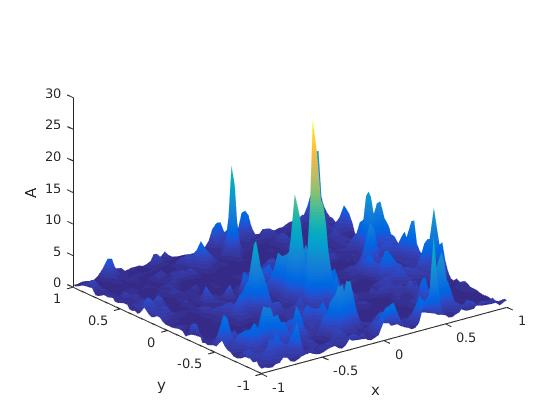
\includegraphics [width=1\linewidth]{Darcy/Pictures/A.jpg}
        \caption{Random field.}
        \label{fig:DarcyA}
    \end{subfigure}
    \begin{subfigure}{0.49\linewidth}
        \centering
        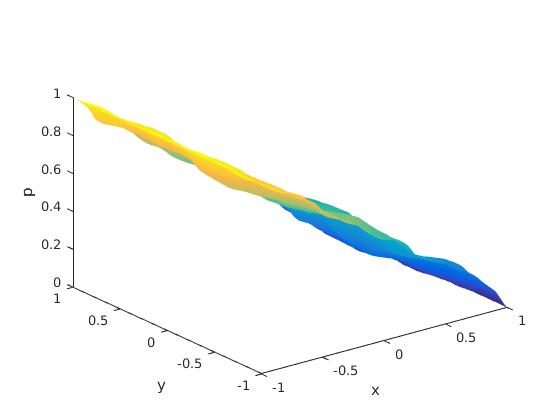
\includegraphics [width=1\linewidth]{Darcy/Pictures/P.jpg}
        \caption{Pressure field.}
        \label{fig:DarcyP}
    \end{subfigure}    
    \begin{subfigure}{0.49\linewidth}
        \centering
        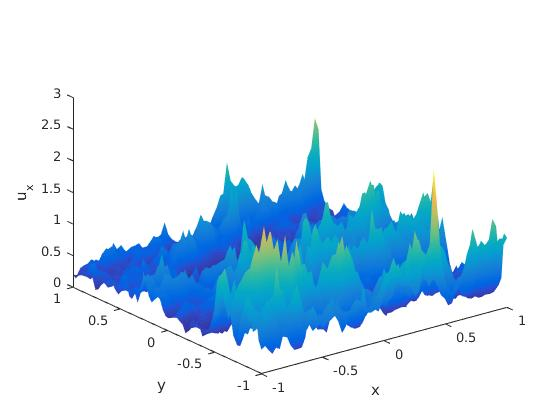
\includegraphics [width=1\linewidth]{Darcy/Pictures/Ux.jpg}
        \caption{$x$ component of velocity field.}
        \label{fig:DarcyUx}
    \end{subfigure}
    \begin{subfigure}{0.49\linewidth}
        \centering
        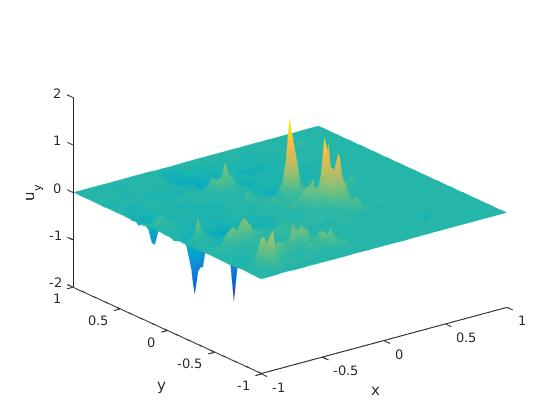
\includegraphics [width=1\linewidth]{Darcy/Pictures/Uy.jpg}
        \caption{$y$ component of velocity field.}
        \label{fig:DarcyUy}
    \end{subfigure}    
    \caption{Approximate solution of the uncertain Darcy problem.}
    \label{fig:DarcyResults}
\end{figure}



\subsection{Finite Elements solution of the Darcy problem}

Let us consider the domain $D = [-1,1] \times [-1,1]$. The random field $A$ in \eqref{eq:DarcyProblem} is chosen to be lognormal, \textit{i.e.}, 
\begin{equation}\label{eq:RandomField}
	A = e^\gamma,
\end{equation}
where $\gamma$ is a normal random field defined by its covariance function $\mathrm{cov}_\gamma(x_1,x_2)$ for any couple of points $x_1,x_2$ in the domain $D$. The covariance function is of the Matern family, thus having the following form
\begin{equation}\label{eq:CovFunction}
	\mathrm{cov}_\gamma(x_1,x_2) = \frac{\sigma^2}{\Gamma(\nu)2^{\nu-1}}\Big(\sqrt{2\nu}\frac{|x_1-x_2|}{L_c}\Big)^\nu K_{\nu}\Big(\sqrt{2\nu}\frac{|x_1-x_2|}{L_c}\Big), \quad \nu \geq 0.5,
\end{equation}
where $\sigma^2$ is the variance, $L_c$ is the correlation length, $\Gamma$ is the gamma function, $K_\nu$ is the modified Bessel function of the second kind and $\nu$ is a parameter. Let us remark that the covariance function does not depend on $x_1, x_2$ but only on their euclidean distance $|x_1 - x_2|$. The regularity of the covariance function and of the realizations of $A$ depend on $\nu$. In particular, for $\nu$ equal to 0.5, the covariance is Lipschitz continuous and the field is $\alpha$-Hölder continuous for $\alpha < 0.5$. Results concerning regularity properties of $A$ can be found in \cite{Nobile2015}. The realizations of $A$ are computed using a discrete Fourier transformation on the vertices of a grid of $D$, equispaced on both the $x$ and $y$ directions with the same spacing $\Delta_A$. Then, the numerical solution $p_h$ of \eqref{eq:DarcyProblem} is obtained with linear Finite Elements on a regular mesh $T_p$ with maximum element size $\Delta_p$. Since the vertices of the grid on which we compute $A$ do not coincide with the vertices of $T_p$, we interpolate $A$ on $T_p$ to obtain $p_h$. Then, the velocity field $u_h$ is retrived computing the gradient on $p_h$. The results for a realization of $A$ are shown in Figure \ref{fig:DarcyResults}, where the value of the inlet pressure $p_0$ is equal to 1, and the parameters for the random field are $\nu = 0.5, L_c = 0.05$. 


\section{Conclusion}

We investigated the stochastic particle transport problem in the framework of underground flow. In particular, we analysed three numerical schemes that allow estimating the exit time of the solution of a general SDE from a bounded domain. Numerical experiments show that CEM seems to be the most appropriate choice in order to fulfill this purpose. In fact, estimating the probability of exit at each timestep using the Brownian bridge approach implies a small computational cost and improves dramatically the precision of DEM. On the other hand, an adaptivity procedure we analysed based on the position of the trajectory in the domain succeeds in restoring the weak order of the Euler-Maruyama scheme in an unbounded domain but does not imply a considerable advantage in computational time. Then, we managed to prove the properties of convergence of the analytic and numerical solution of a perturbed SDE to its non-perturbed solution. This is fundamental when an interpolation of the transport field is needed to increase computational speed. The convergence is confirmed by numerical results on a test case, where we succeeded in tuning the parameters of interpolation and time integration in order to have good performances. Finally, we applied the numerical schemes to the Darcy case, providing the details of a double Montecarlo simulation that can be exploited to estimate the exit time of a pollutant particle in the frame of the underground flow problem. Future improvements of the procedure explained in this work could be done employing Multi Level Montecarlo techniques for estimating the exit time in the Darcy case. Moreover, the modeling of extraction wells has not been taken into account, since we feel that the integration of the SDE in presence of singularities in the velocity field would have implied a deeper theoretical investigation and different numerical techniques.  

	
\end{document}
